%
%            ,,,                                        
%          `7MM            _.o9                                
%            MM                                             
%  ,6"Yb.    MM  ,p6"bo   ,6"Yb.  M"""MMV  ,6"Yb.  `7Mb,od8 
% 8)   MM    MM 6M'  OO  8)   MM  '  AMV  8)   MM    MM' "' 
%  ,pm9MM    MM 8M        ,pm9MM    AMV    ,pm9MM    MM     
% 8M   MM    MM YM.    , 8M   MM   AMV  , 8M   MM    MM     
% `Moo9^Yo..JMML.YMbmd'  `Moo9^Yo.AMMmmmM `Moo9^Yo..JMML.   
%
%
% Chapter 3: Loss Functions

\clearpage
\cleardoublepage

\chapter{Loss Functions}

\section{Introduction}

Loss functions (also called objective functions, cost functions, or error functions) are the mathematical measures that quantify how well a neural network's predictions match the true targets. The training process aims to minimize this loss by adjusting the network's parameters through gradient-based optimization.

The choice of loss function depends on:
\begin{itemize}
    \item The type of task (classification, regression, etc.)
    \item The distribution of the target variable
    \item The desired properties of the solution (sparsity, robustness, etc.)
    \item Computational considerations
\end{itemize}

\section{The Role of Loss Functions}

Given a dataset $\mathcal{D} = \{(\mathbf{x}_i, \mathbf{y}_i)\}_{i=1}^{N}$ and a model $f(\mathbf{x}; \mathbf{\theta})$, the empirical risk is:
\begin{equation}
\mathcal{R}(\mathbf{\theta}) = \frac{1}{N}\sum_{i=1}^{N} \ell(f(\mathbf{x}_i; \mathbf{\theta}), \mathbf{y}_i)
\end{equation}
where $\ell(\cdot, \cdot)$ is the loss function.

Training seeks to find:
\begin{equation}
\mathbf{\theta}^* = \arg\min_{\mathbf{\theta}} \mathcal{R}(\mathbf{\theta})
\end{equation}

The loss function should:
\begin{enumerate}
    \item Be differentiable (for gradient-based optimization)
    \item Penalize larger errors appropriately
    \item Encourage correct behavior for the specific task
    \item Have useful statistical interpretations
\end{enumerate}

\section{Regression Loss Functions}

Regression tasks predict continuous values.

\subsection{Mean Squared Error (MSE)}

The Mean Squared Error (L2 loss):
\begin{equation}
\mathcal{L}_{MSE} = \frac{1}{N}\sum_{i=1}^{N} \|\mathbf{y}_i - \hat{\mathbf{y}}_i\|^2
\end{equation}

\begin{properties}[Properties of MSE]
\begin{itemize}
    \item \textbf{Gradient:} $\frac{\partial \ell}{\partial \hat{y}} = -2(\mathbf{y} - \hat{\mathbf{y}})$
    \item \textbf{Convex for linear models}
    \item \textbf{Sensitive to outliers}
\end{itemize}
\end{properties}

\begin{figure}[h]
    \centering
    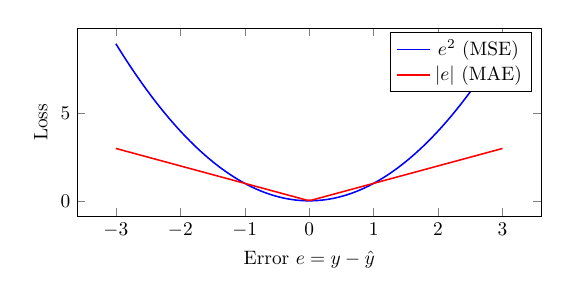
\begin{tikzpicture}[scale=0.7]
        \begin{axis}[
            xlabel={Error $e = y - \hat{y}$},
            ylabel=Loss,
            domain=-3:3,
            samples=100,
            width=10cm,
            height=5cm
        ]
            \addplot[thick, blue] {x^2};
            \addlegendentry{$e^2$ (MSE)}
            \addplot[thick, red] {abs(x)};
            \addlegendentry{$|e|$ (MAE)}
        \end{axis}
    \end{tikzpicture}
    \caption{MSE vs MAE loss functions}
    \label{fig:mse_mae}
\end{figure}

\subsection{Mean Absolute Error (MAE)}

The Mean Absolute Error (L1 loss):
\begin{equation}
\mathcal{L}_{MAE} = \frac{1}{N}\sum_{i=1}^{N} \|\mathbf{y}_i - \hat{\mathbf{y}}_i\|_1
\end{equation}

Robust to outliers but non-differentiable at zero.

\subsection{Huber Loss}

Combines MSE and MAE:
\begin{equation}
\mathcal{L}_{\text{Huber}}(y, \hat{y}) = 
\begin{cases}
\frac{1}{2}(y - \hat{y})^2 & \text{if } |y - \hat{y}| \leq \delta \\
\delta \cdot |y - \hat{y}| - \frac{1}{2}\delta^2 & \text{otherwise}
\end{cases}
\end{equation}

\section{Classification Loss Functions}

Classification tasks predict discrete class labels.

\subsection{Binary Cross-Entropy}

For binary classification ($y \in \{0, 1\}$):
\begin{equation}
\mathcal{L}_{BCE} = -\frac{1}{N}\sum_{i=1}^{N}[y_i \log \hat{y}_i + (1-y_i) \log(1-\hat{y}_i)]
\end{equation}

where $\hat{y}_i = \sigma(\mathbf{w}^\top \mathbf{x}_i + b)$.

\begin{advantages}
    \item Probabilistic interpretation
    \item Equivalent to MLE for binary classification
    \item Strong gradients even for confident wrong predictions
\end{advantages}

\subsection{Categorical Cross-Entropy}

For multi-class classification:
\begin{equation}
\mathcal{L}_{CE} = -\frac{1}{N}\sum_{i=1}^{N}\sum_{k=1}^{K} y_{ik} \log \hat{y}_{ik}
\end{equation}

where $\hat{y}_{ik} = \text{softmax}(z_{ik})$.

A key property is the gradient:
\begin{equation}
\frac{\partial \mathcal{L}}{\partial z_k} = \hat{y}_k - y_k
\end{equation}

\section{Advanced Loss Functions}

\subsection{Focal Loss}

Addresses class imbalance in object detection:
\begin{equation}
\mathcal{L}_{\text{Focal}} = -\alpha_t (1 - \hat{y}_t)^\gamma \log(\hat{y}_t)
\end{equation}

where $\gamma \geq 0$ focuses training on hard examples.

\subsection{Label Smoothing}

Regularizes by softening hard labels:
\begin{equation}
y_{LS} = y(1 - \epsilon) + \frac{\epsilon}{K}
\end{equation}

where $\epsilon \in [0, 1]$ is the smoothing parameter.

\section{Specialized Loss Functions}

\subsection{Triplet Loss}

For metric learning:
\begin{equation}
\mathcal{L}_{\text{Triplet}} = \max(0, \|f_a - f_p\|^2 - \|f_a - f_n\|^2 + \alpha)
\end{equation}

Ensures positive pairs are closer than negative pairs by margin $\alpha$.

\subsection{Dice Loss}

For segmentation tasks:
\begin{equation}
\mathcal{L}_{\text{Dice}} = 1 - \frac{2|A \cap B|}{|A| + |B|}
\end{equation}

Handles class imbalance in segmentation.

\section{Choosing a Loss Function}

\begin{table}[h]
    \centering
    \caption{Loss Function Selection Guide}
    \begin{tabular}{L{2.5cm} L{4cm} L{4cm}}
        \toprule
        \textbf{Task} & \textbf{Loss} & \textbf{Notes} \\
        \midrule
        Binary Classification & BCE & Standard choice \\
        Multi-class & Cross-Entropy & With label smoothing \\
        Regression & MSE & Sensitive to outliers \\
        Robust Regression & MAE/Huber & Outlier resistant \\
        Imbalanced Classification & Focal Loss & Focus on hard examples \\
        Segmentation & Dice + CE & Handle class imbalance \\
        \bottomrule
    \end{tabular}
\end{table}

\section{Chapter Summary}

Loss functions are fundamental to neural network training:
\begin{enumerate}
    \item MSE is standard for regression but sensitive to outliers
    \item Cross-entropy is standard for classification
    \item Advanced losses address specific challenges like class imbalance
    \item Label smoothing provides regularization
    \item Task-specific losses exist for segmentation and metric learning
\end{enumerate}

\section{Further Reading}

\begin{itemize}
    \item Goodfellow et al., ``Deep Learning'' Chapter 6
    \item Lin et al., ``Focal Loss for Dense Object Detection'' (ICCV 2017)
    \item Milletari et al., ``V-Net'' (MICCAI 2016)
\end{itemize}
